%!TEX program = xelatex

% Name           : coq-hsrm-beamer-minimal.tex
% Author         : Tanja Almeroth (tanja.almeroth@mailbox.org)

% Copyright      : Copyright (c) 2020 by Tanja Almeroth. All rights reserved.
% License        : This file may be distributed and/or modified under the
%                  GNU Public License.
% Build up on the: HSRM beamer theme minimal example.
%                  (https://github.com/benjamin-weiss/hsrmbeamertheme)

% syntaxhighlighting for Gallina (Coq) listings
% see (https://github.com/nickgian/thesis)

\documentclass{beamer}
\graphicspath{{pics/}} % searchpath for graphics
\usepackage[english]{babel}
\usepackage{multicol}
%Erweiterte Tabellenfunktionen
\usepackage{tabularx,ragged2e}
\usepackage{booktabs}
% Listingserweiterung




\usepackage{listings}
\usepackage{lstcoq}
\lstset{language=coq, % Coq
		tabsize=4, % Tabulatorbreite
		linewidth=\linewidth, % Width of a line
		breaklines=true, % Break long lines
		breakatwhitespace=true, % Only break at whitespaces
		basicstyle=\scriptsize\ttfamily, % Schriftart/-größe
		numbers=left, % Linenumbers left
		numberfirstline=false, % Not: Always number 1. line
		numberstyle=\scriptsize, % Größe der Zeilennummern
		stepnumber=1, % Jede 2. Zeilennummer anzeigen
		numbersep=5pt, % Abstand Nr - Quellcode
		showspaces=false, % Spaces nicht anzeigen
		showtabs=false, % Tabs nicht anzeigen
		showstringspaces=false, % Don't show tabs in strings
		showlines=false, % Leerzeilen am Sourceende weglassen
		extendedchars=true, % ASCII-Zeichnen > 127 zulassen
		identifierstyle=\bfseries, % Identifier
		keywordstyle=\bfseries, % Keywords
		commentstyle=\itshape, % Style of comments
		stringstyle=\ttfamily, % Strings (!= Keywords)
		flexiblecolumns=false, % Use fixed width for fonts
		fontadjust=true, % "Base width" nicht jede Zeile anpassen
		frame=trbl, % Frame; trBL
		captionpos=b, % Position of the caption
		aboveskip=25pt}% Space between text and the top of the listing
		
%----------------------------------------------------------------------
% Load theme
\usetheme{hsrm}
%----------------------------------------------------------------------

% see slide logic using tikzpicture
%\usepackage{dtklogos} % must be loaded after theme
%\usepackage{tikz}
%\usetikzlibrary{mindmap,backgrounds}

%claim environment
\newenvironment{claim}[1]{\par\noindent\underline{Claim:}\space#1}{}
\newenvironment{claimproof}[1]{\par\noindent\underline{Proof:}\space#1}{\hfill $\blacksquare$}

%-----------------------------------------------------------------------
% title page
\title{A Brief Introduction To Coq}
\subtitle{The Coq Proof Assistant}
\author{Tanja Almeroth}
\institute{Studienbereich DCSM\\Hochschule {\Medium RheinMain}}
\date{\today}


\begin{document}
	
	\maketitle
		
% table of contents
	\section*{table of contents}
	
		\begin{frame}
			\frametitle{table of contents}
			\tableofcontents[hideallsubsections]
		\end{frame}
	
	
% start of presentation 


% section about proof assitants	
	\section{proof assistants}
	
	\begin{frame}{The Coq Proof Assistant}
	
		\begin{columns}[t]
			\begin{column}{8cm}
			usage and applicability of the Coq-proof-assistant
	
			\begin{itemize}
			\item developed since 1983
			\item community in the industry and research
			       \url{https://coq.inria.fr/community}
				   \url{https://github.com/coq-community}
		
			\end{itemize}
			
		    \begin{itemize}
			\item basic concepts of logic
			\item functional programming
			\end{itemize}
		\end{column}
		\begin{column}{2.5cm}
			\begin{figure}[h]
			
\includegraphics[width=.9\textwidth]{barron_logo.png} 
			\label{coq_rorster}
			\caption[c]{The Rooster. Source:\cite{COQ}}
			\end{figure}
		\end{column}
		\end{columns}
		
	\end{frame}
	
	
	\begin{frame}{Other Proof Assistants}
	
			There are numerous proof assistants.
	
			\begin{itemize}
			\item Isabelle \\
			      \url{https://isabelle.in.tum.de}
			\item HOL \\
			       \url{https://hol-theorem-prover.org}		
			\end{itemize}
		
	\end{frame}
	
	
	\begin{frame}{Logic}
	
		\begin{quote}
		`'As as matter of fact, logic has turned out to be significantly more effective in computer science then it has been in mathematics.''
		\cite{PACGGHSY2019}
		\end{quote}
		
	\end{frame}
	
	
	
	\begin{frame}{logic}
		Reliability in software is amplified by the costs of bugs by insecurity up to multiple levels.


% Could not make this build although I have TExLive installed.
% I would be nice for the people without mathematical skills, to visualize this slide differntly.
%
%		centering
%\begin{tikzpicture}[scale=0.88]
	%\tikzset{every child/.append style={level distance=250}}
%	\path[mindmap,concept color=hsrmWarmGreyLight,text=hsrmWarmGreyDark]
%	node[concept] {\TeX}
%	[clockwise from=-30]
%	child[concept color=hsrmSec2Dark,text=white] { node[concept] {\textcolor{white}{\XeTeX}} }
%	child[concept color=hsrmSec1CompDark,text=white] { node[concept] {\ConTeXt} }
%	child[concept color=hsrmSec1Dark,text=white] { node[concept] {\LaTeX} };
%\end{tikzpicture}
		\begin{itemize}
			\item basic tools from logic
			\item precise claims about programs
			\item functional programming methods of programming and logical reasoning about programs
		\end{itemize}
	\end{frame}
	
%---------------------------------------------------------------------------------------
%
% section about functional programming in COQ 
%	
%---------------------------------------------------------------------------------------	


	\section{functional programming in coq}
	
	\begin{frame}[containsverbatim]{System Requirements}
		Coq runs on Linux, Mac OS and Windows.\\
		There are a lot of development environments available.
			\begin{itemize}
				\item \alert{Proof General}\\
						 an Emacs based IDE\\
				\item \alert{CoqIDE}\\ 
						is a simple stand-alone IDE
				\item \alert{coquille} \\
						a vim plug-in 
				\item and others
			\end{itemize}
	\end{frame}
	
	
	\begin{frame}[containsverbatim]{System Requirements}
		Coq runs on Linux, Mac OS and Windows.\\
		There are a lot of development environments.
			\begin{itemize}
				\item \alert{Proof General}\\
						 an Emacs based IDE\\
						 generic interface for proof assistants developed by multiple universities						 
				\item \alert{CoqIDE}\\ 
						is a simple stand-alone IDE\\
						user-friendly, included in the official Coq-installation
				\item \alert{coquille} \\
						a vim plug-in\\
						an open-source project
			\end{itemize}
	\end{frame}
	
	%
	% Which one is the most trustable proof checker? 
	%
	
	\begin{frame}{Proof General}
		\begin{figure}[h]
			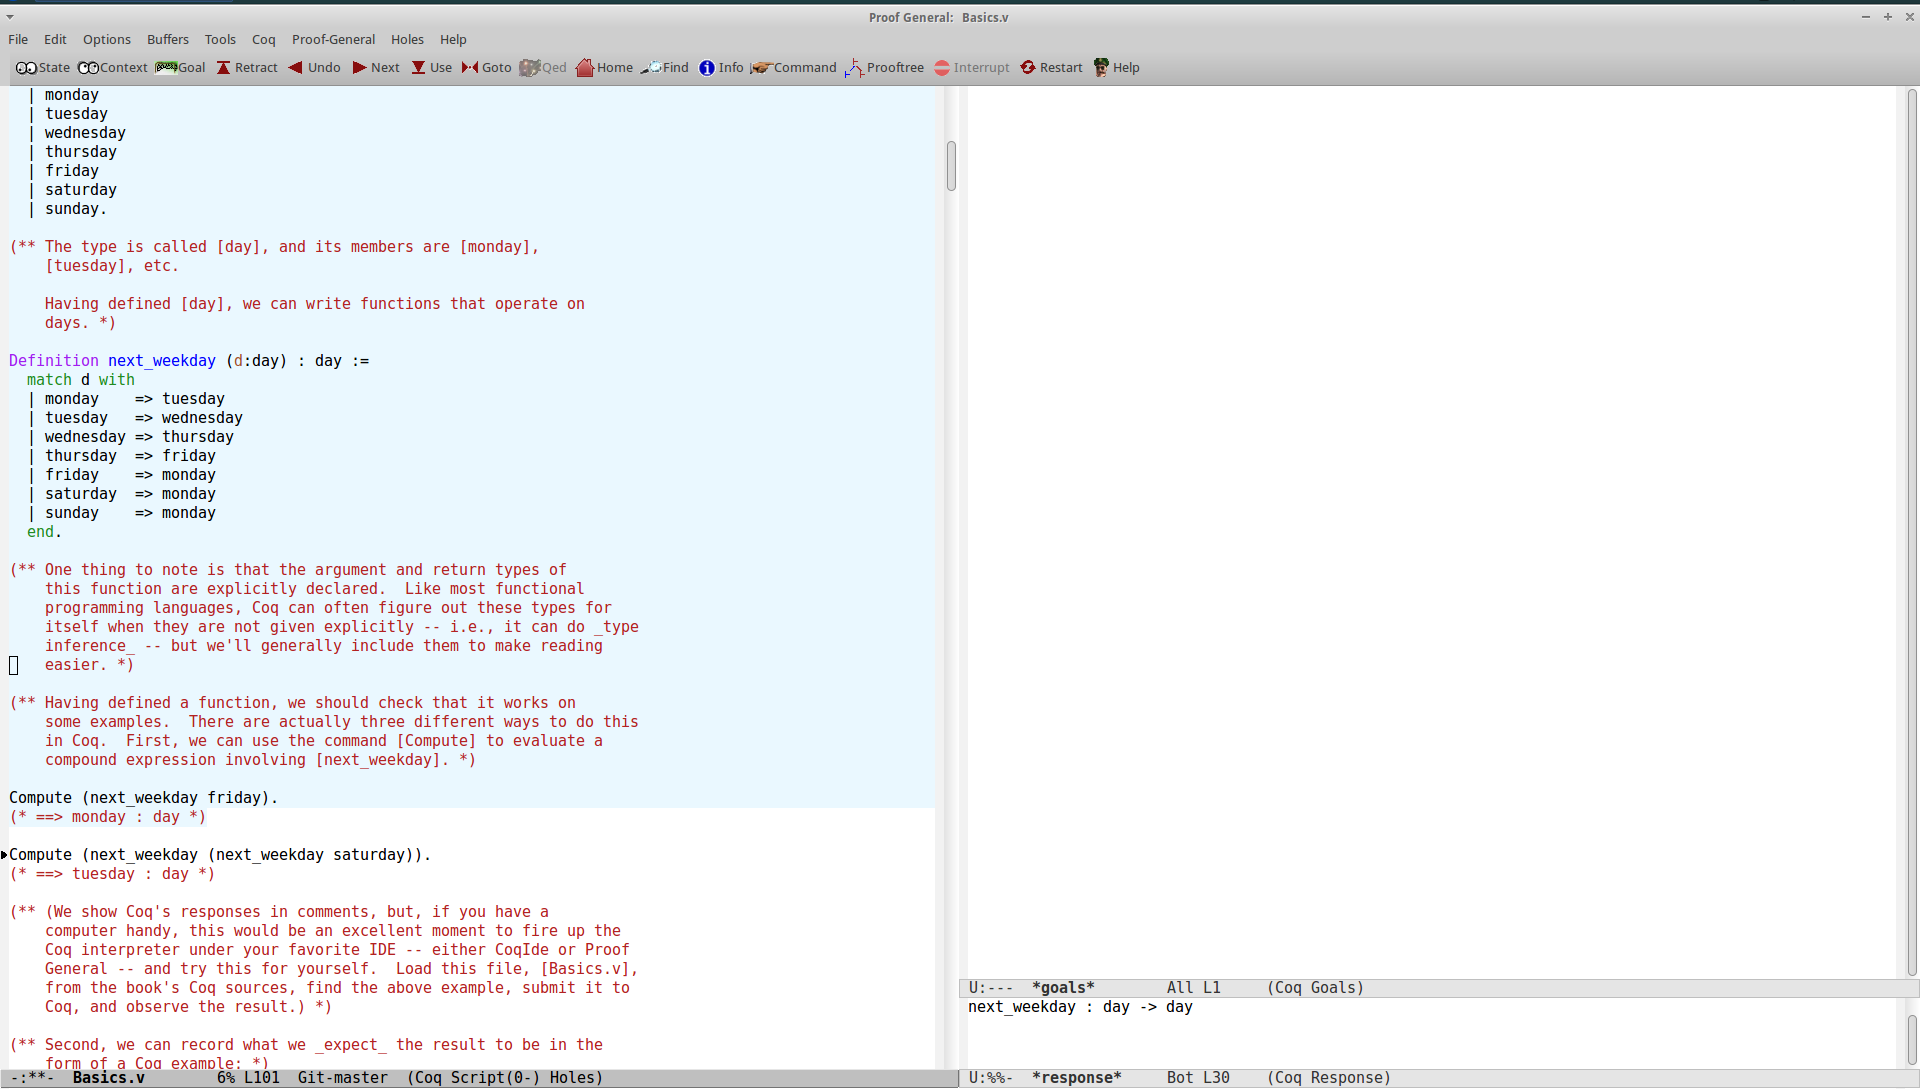
\includegraphics[width=.9\textwidth]{proofgeneral.png}
			\label{fig:screenshot-proof-general}
			\caption{Coq interface in proof general.}
		\end{figure}
	\end{frame}
	
	\begin{frame}{CoqIDE}
	\begin{figure}[h]
			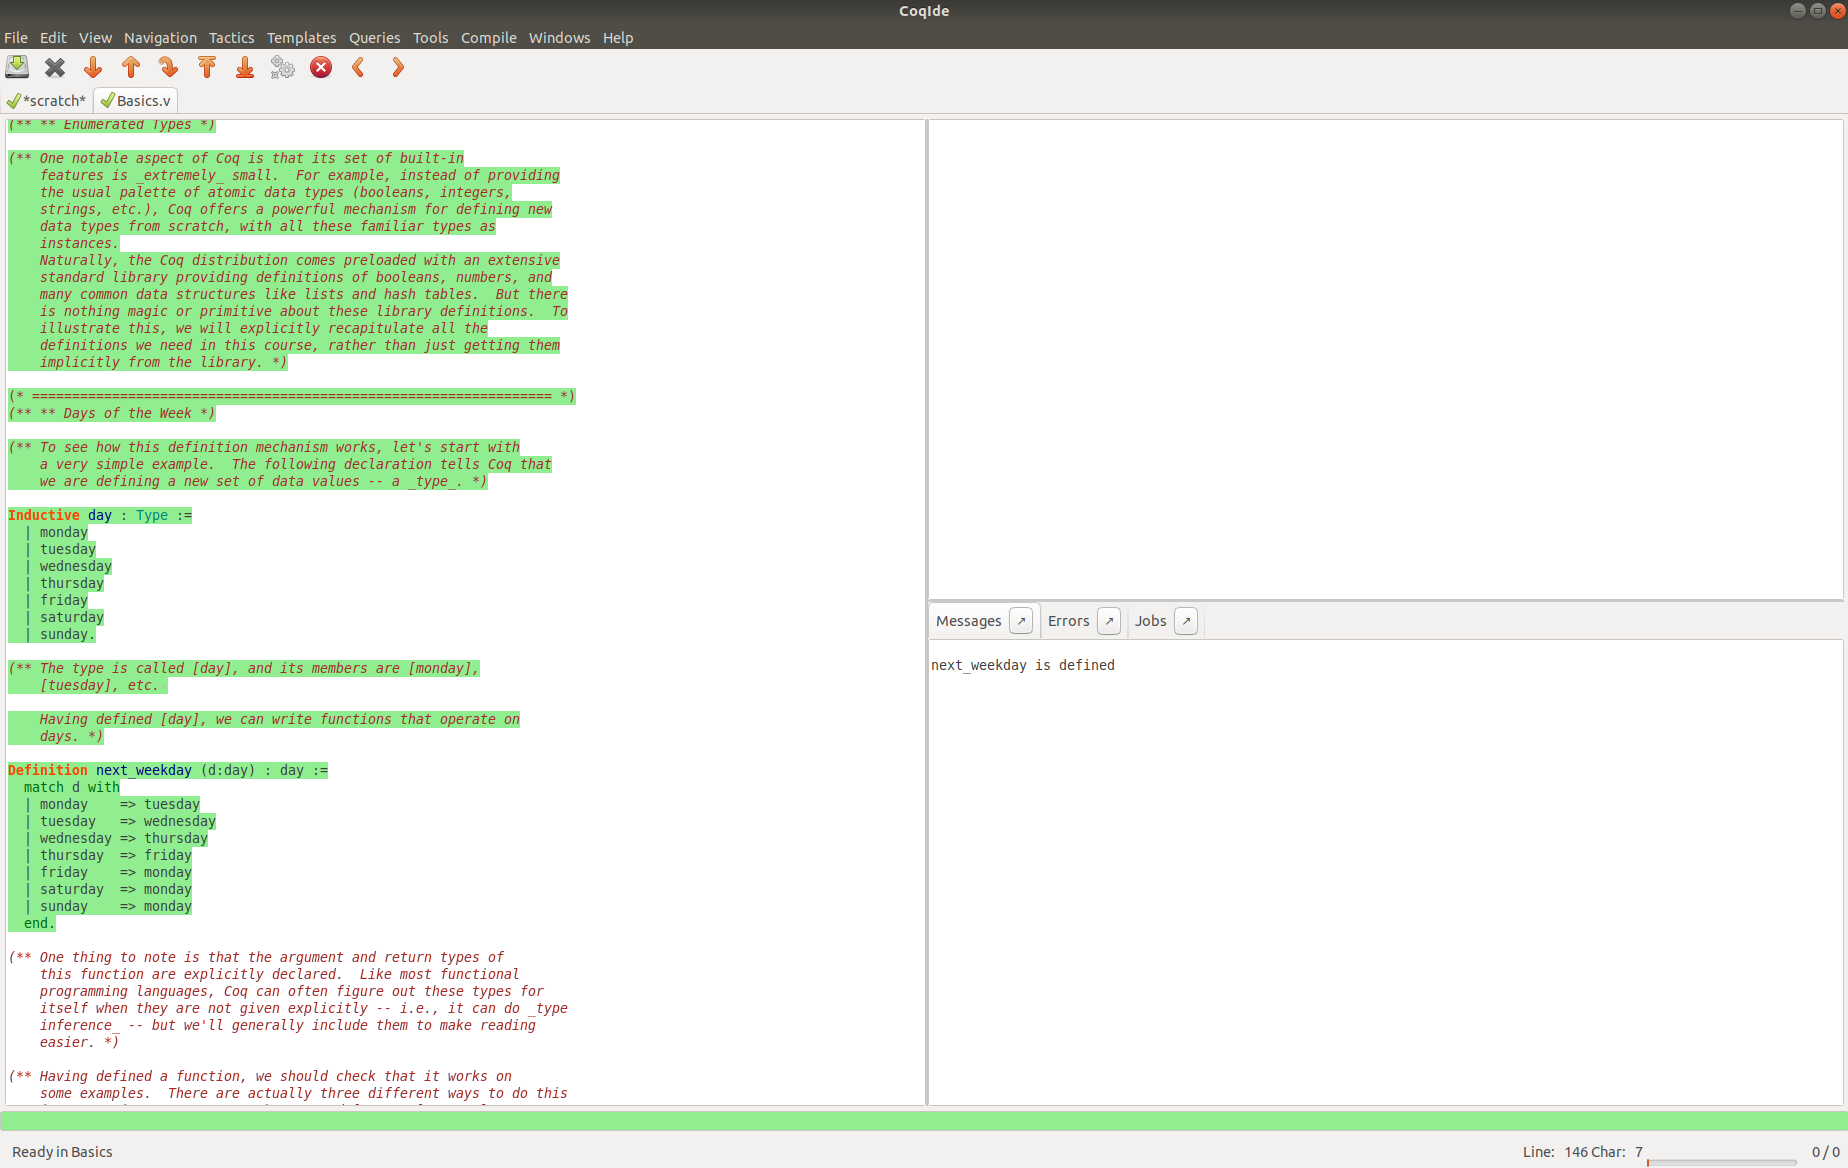
\includegraphics[width=.9\textwidth]{coqide.png}
			\label{fig:screenshot-coqide}
			\caption{Coq interface in CoqIDE.}
			\end{figure}
	\end{frame}
	
	\begin{frame}{Coquille}
	\begin{figure}[h]
			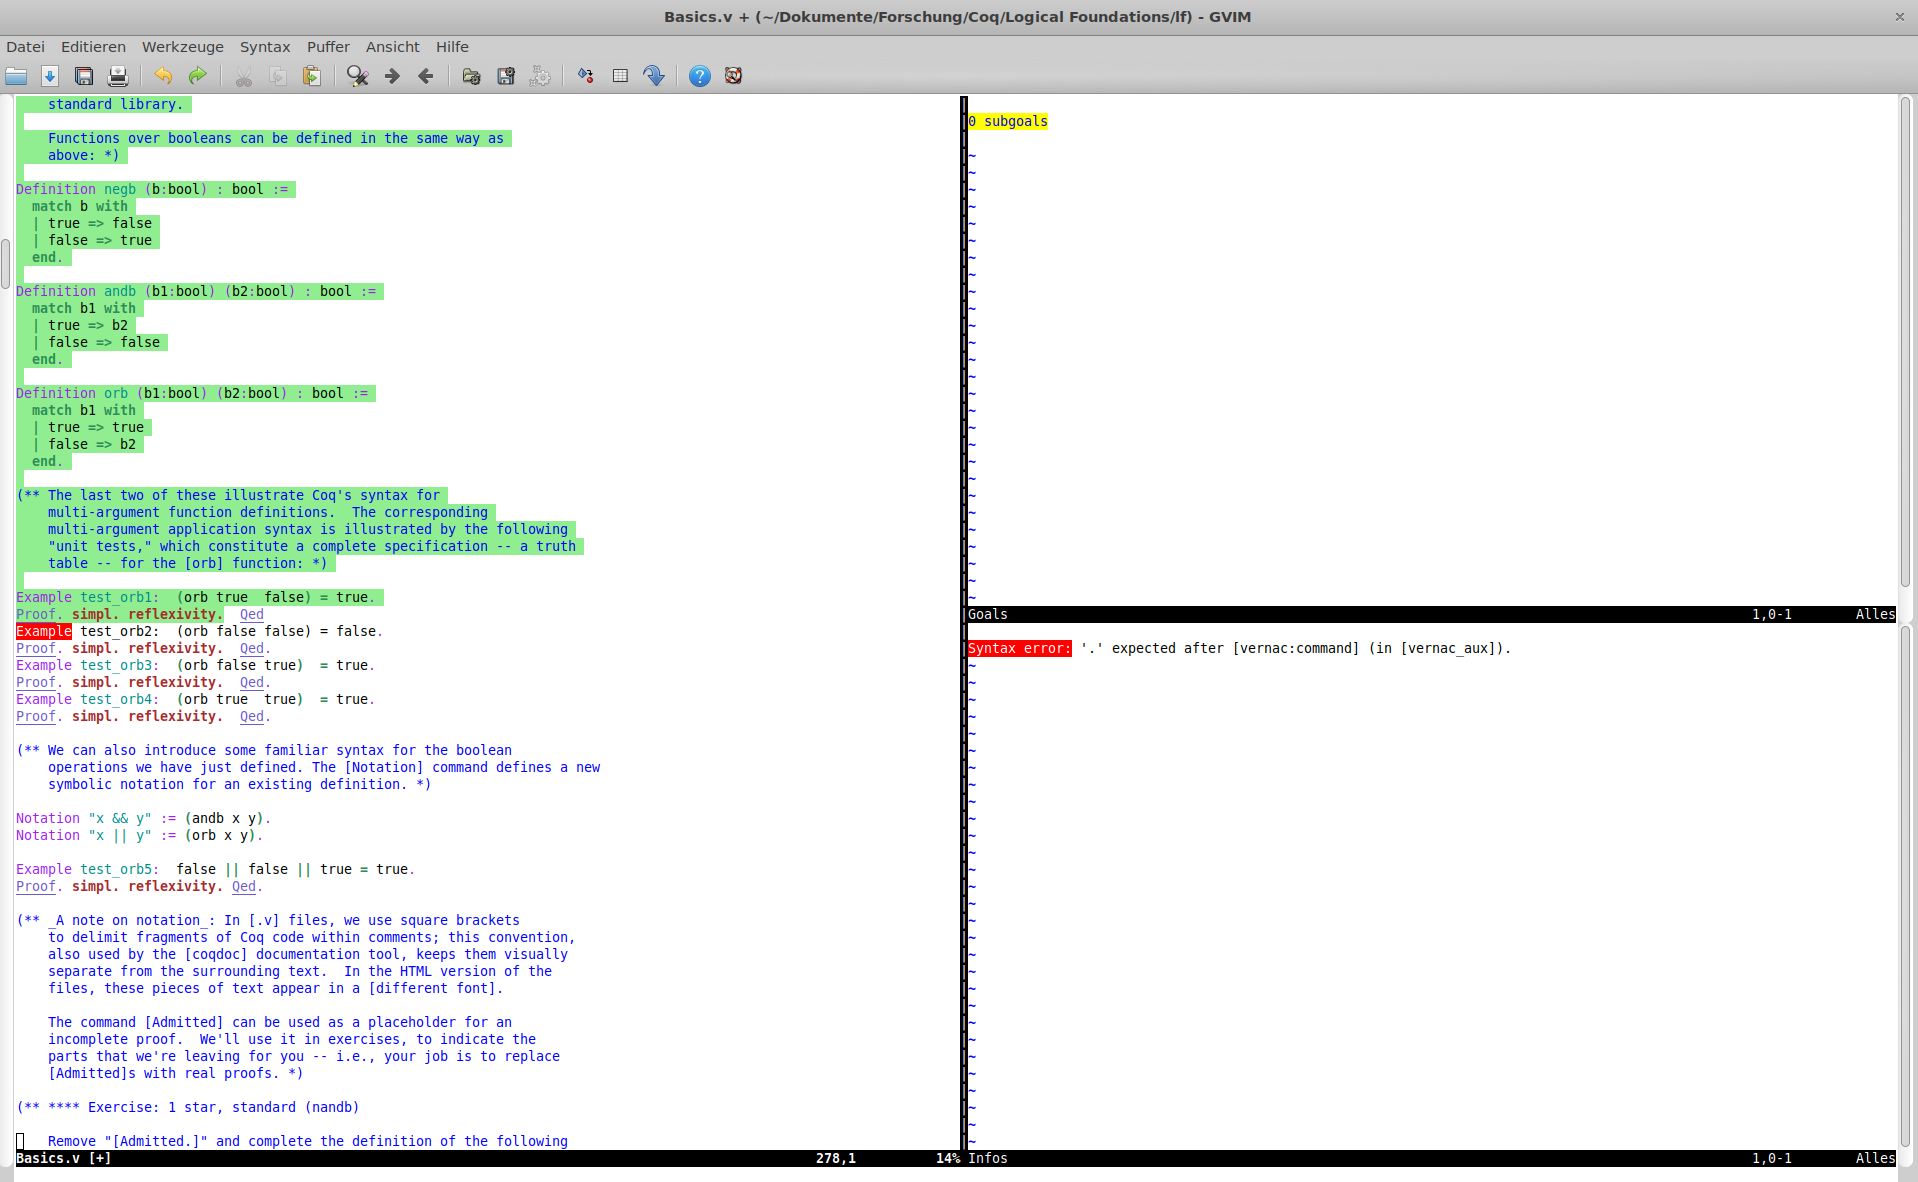
\includegraphics[width=.9\textwidth]{coquille.png}
			\label{fig:screenshot-coquille}
			\caption{Coq interface in gvim using coquille.}
			\end{figure}
	\end{frame}
	
	
	\begin{frame}{functional programming}
		Coq's functional programming language {\itshape Gallina's}\\
		sub-types
			\begin{enumerate}
				\item vernacular language (top-level interaction):\\
					  e.g.: \lstinline!Theorem!, \lstinline!Proof!, \lstinline!Qed!.
				\item tactics language:\\
				e.g.: \lstinline!intros!, \lstinline!exact!\\
				 	
			\item the {\itshape language of Coq-terms}:\\
				e.g.:  \lstinline!for all A: Prop, A -> A.! 
			\end{enumerate}
	\end{frame}
	
	
	
%%%%%%%%%%%%%%%%%%%%%%%%%%%%%%%%%%%%%%%%%%%%	
% section programming in Coq	
%%%%%%%%%%%%%%%%%%%%%%%%%%%%%%%%%%%%%%%%%%%%
	
	\section{an example}
	
	
	% have to define lstlistings for below due to usage of a framed box
	% see verbatim documentation 
	
	
	% an example definition in Gallina of a new datatype	
	\defverbatim[colored]\CoqDef{%
	\begin{lstlisting}[frame=single, emph={cout}, emphstyle=coq, label = lst:TypeDay, caption = definition of a  datatype called \lstinline!day!]
	Inductive day : Type :=
	  | monday
	  | tuesday
	  | wednesday
	  | thursday
	  | friday
	  | saturday
	  | sunday.
	\end{lstlisting} 
	}

	
	% an example definition of a Gallina function 
	\defverbatim[colored]\CoqFunc{%
	\begin{lstlisting}[frame=single, emph={cout}, emphstyle=coq, label = lst:DefFunc, caption = declaration of a function on \lstinline!day!]
		Definition next_weekday (d:day) : day :=
	  		match d with
	  		| monday    => tuesday
	  		| tuesday   => wednesday
	  		| wednesday => thursday
	  		| thursday  => friday
	 	    | friday    => monday
	  		| saturday  => monday
	  		| sunday    => monday
	  		end.
		\end{lstlisting} 
	}
	
	
	% an example computation in Gallina	
	\defverbatim[colored]	\CoqCompute{
	\begin{lstlisting}[frame=single, emph={cout}, emphstyle=coq, label = lst:compute, caption = call \lstinline!Compute! ]
	Compute (next_weekday friday).
	\end{lstlisting}
	\begin{lstlisting}[frame=single, emph={cout}, emphstyle=coq, label = lst:output, caption = output ]
	= monday: day 
	\end{lstlisting} 
	}
	

	 % make slides	
	
	\begin{frame}{an example}
	\CoqDef % type weekday
	\end{frame}
	% we defined a new type called weekday
  
	\begin{frame}{an example}
	\CoqFunc % next_weekday
	\end{frame}
	% We defined a function in coq on our new type called day.
	
	\begin{frame}{an example}
	\CoqCompute % example calculation
	\end{frame}	
	% We computed something. E.g. called our first data type and function by name.
	% This is dynamic type reference in Coq. 
	% An 'std::cout>>"Hallo World";' in Coq.  


%%%%%%%%%%%%%%%%%%%%%%%%%%%%%%%%%%%%%%%%%%%%%%%%%%%%
% Applications
%%%%%%%%%%%%%%%%%%%%%%%%%%%%%%%%%%%%%%%%%%%%%%%%%%%%

	
	\section{applications}
	
	
	\begin{frame}{applications}
		 A platform for {\itshape modeling programming languages} and an environment for {\itshape formally certifying software and hardware}
	     \begin{itemize}
	     \item PROSA a felxible open-source foundation for formally proven schedulability analysis. PROSA uses the Coq proof assistant and the SSREFLECT extension library \cite{PROSA_ECRTS16ArtifcatEvaluation} 
	     \item Jasmin: High-Assurance and High-Speed Cryptography \cite{JASMIN}
	     \end{itemize}
	\end{frame}
	
%%%%%%%%%%%%%%%%%%%%%%%%%%%%%%%%%%%%%%%%%%%%%%%%%%%%%%%%
% PROSA
%%%%%%%%%%%%%%%%%%%%%%%%%%%%%%%%%%%%%%%%%%%%%%%%%%%%%%%%	
	
	\section{PROSA}
	
	\begin{frame}{PROSA - a Coq library}
		\begin{figure}[h]
			
\includegraphics[width=.4\textwidth]{logo_RT-proofs.png}
			\label{fig:RT-proofs-logo}
			\caption{RT-proofs-logo. Source: \cite{RTproofs}.} %
		\end{figure}
		\begin{enumerate}
			\item Formal Proofs for real-time systems (RT-Proofs)
			\item project running between multiple research faculties\\
			  (DFG project between INRIA, MPI-SWS, Onera, TU Braunschweig and Verimag, running from 2018 until 2020)
			\item The PROSA library is where this development takes place.%
		\end{enumerate}	
	\end{frame}
	
	% listing in bashstyle about a VM
	\defverbatim[]\PROSAVM{%		
	\begin{lstlisting}[language=bash, frameround=fttt, label = lst:PROSA_environment]
			Coq Version 8.5
			mathcomp-1.6
			PROSA v01.zip
			Proof General Version 4.3pre131011
		    VM-Image: Ubuntu 15.10, wily
		    Bertonas .. and ...		
      \end{lstlisting}
      } 
          
      
      
      \begin{frame}{PROSA - a Coq library}
		to reproduce the PROSA - ECRTS’16 Artifact Evaluation by mechanically proofing the case study the following framework is provided online
		\begin{table}[]
			\begin{tabularx}{\linewidth}{l>{\raggedright}X}
				\textbf{utility}         & source				\tabularnewline
				\bottomrule
				\texttt{Ubuntu 15.10, wily}& VM-Image   			\tabularnewline           
				\texttt{Coq Version 8.5pl}   & VM-Image                    \tabularnewline                    
				\texttt{Proof General 4.3pre131011}		& VM-Image  \tabularnewline				
				\texttt{mathcomp-1.6}, \texttt{ssreflect}-extension	   & VM-Image \tabularnewline
				\bottomrule
				\texttt{PROSA v.01}		& former version of the Coq spec and proof development of the RT-PROOFS project\tabularnewline
				\bottomrule
			\end{tabularx}
			\label{tab:PROSA setup}
		\end{table}			 
      \end{frame}
      
      % As written on the PROSA-ECRTS'16 Artifact evaluation website:
      
      % Note that any required packages for Coq should be installed by your linux. 
      % Only the ssreflect installation is required not the complete mathematical componets library.
      % build prosa by '$ make -j4' then look at it
  	  % '$ make validate' runs the proof checker
  	  % If this comand is proceded without errors or warnings, the proof is machine checked. 
  	  
  	 \begin{frame}{PROSA - a Coq library}
		to reproduce the PROSA - ECRTS’16 Artifact Evaluation by mechanically proofing the case study the following framework is provided online
		\begin{table}[]
			\begin{tabularx}{\linewidth}{l>{\raggedright}X}	
			my current working directory:\tabularnewline
			\url{https://gitlab.cs.hs-rm.de/almeroth/prosa_working_dir}\tabularnewline
			members: Steffen Reith \tabularnewline 
			due to documentation including all listings		
			\end{tabularx}
			\label{tab:Prosa_working_Dir}
		\end{table}			 
      \end{frame}  

% Explain what PROSA wants.
      
      
      
	\defverbatim[colored]\PROSAmaintheorem{%		
		\begin{lstlisting}[emphstyle=coq, label = lst:theorem_edf_analysis, caption = \lstinline!theorem_edf_analysis! \cite{PROSA_ECRTS16ArtifcatEvaluation}]
			Theorem edf_analysis_yields_response_time_bounds :
        		∀ tsk R,
          		(tsk, R) \\In edf_claimed_bounds ts →
          		response_time_bounded_by tsk R. 
		\end{lstlisting}
      }       
    
    
	\begin{frame}{PROSA - formally proven schedubility analysis}
	
		\begin{itemize}
			\item \doublequoted{We conclude that the develop foundations are sufficiently felixble and powerful to support a large fraction of existing literature and real-time scheduling, without compromising readability.} \cite{PROSA_ECRTS16ArtifcatEvaluation}\\
			\item \doublequoted{Mechanized schedulability proofs are feasible, to the point that non-trivial 				multiprocessor schedulability analyses can be formalized in a reasonable time frame.}\cite{PROSA_ECRTS16ArtifcatEvaluation}				
			\item \alert{case studies}
		\end{itemize}
	\end{frame}    
      
	
	\begin{frame}{prosa - formally proven schedubility analysis}
	
	\alert{a case study provided}: Ciriniei's RTA for EDF  \cite[p.160, Figure 17.3]{C}\\
	 definition and proofs of termination and correctness of Bertonga and Cicerei's RTA for EDF
		\begin{theorem}[Main Theorem]			
			\PROSAmaintheorem
		\end{theorem} 
		
 	\end{frame}


	
	\begin{frame}{PROSA - formally proven schedubility analysis}
	 	  practical specification: correctness of the proof
	 		   
	   	\begin{block}{mechanized proofs available}
	   	\begin{itemize}
			\item correctness of  the work-loaded-based interference bound  for work-conserving schedulers 
			\item EDF-specific interference bound definition and proof of termination and correctness  of Bertongna and Cicerei's RTA for FP scheduling
			 \item definition and proof of termination and correctness of Bertongna and Cicerei's RTA for EDF scheduling ($\approx 1'320$ LOC)    	   
	   	\end{itemize} 
	    \end{block}	
		$\approx 13'070$ \texttt{LOC}
 	\end{frame}
 	
 	
 	
		\begin{frame}{PROSA - formally proven schedubility analysis}
	 	  practical specification: correctness of the proof
	 		   
		   	\begin{block}{mechanized proofs available}
			   	\begin{itemize}
					\item correctness of  the work-loaded-based interference bound  for work-conserving schedulers 
					\item EDF-specific interference bound definition and proof of termination and correctness  of Bertongna and Cicerei's RTA for FP scheduling
					 \item \alert{definition} \alert{and} \alert{proof} \alert{of} \alert{termination} \alert{and} \alert{correctness} \alert{of} \alert{Bertongna} \alert{and} \alert{Cicerei's} \alert{RTA} \alert{for} \alert{EDF} \alert{scheduling} \\($\approx 1'320$ LOC)    	   
			   	\end{itemize} 
		    \end{block}	
		$\approx 13'070$ \texttt{LOC}
 	\end{frame}
%%%%%%%%%%%%%%%%%%%%%%%%%%%%%%%%%%%%%%%%%%%%%%%%%
% break
%%%%%%%%%%%%%%%%%%%%%%%%%%%%%%%%%%%%%%%%%%%%%%%%% 	
	\section{break}
 	
 	\begin{frame}{Break - Let's talk about inside and outside. }
 	
	 	% make a möbiusstrip with your boss. https://www.wikihow.com/Explore-a-Mobius-Strip
	 	% Inside and outside is not as clear as he thinks it is.
	 	
		\begin{figure}
			\centering
			\includegraphicscopyright[width=0.7\linewidth]{Klein_bottle_translucent.png}{Klein Bottle with slight transparency, rendered with Mathematica 8 using the parameterisation provided by Robert Israel. Copyright by \href{https://en.wikipedia.org/wiki/Klein_bottle}{wikipedia}, \href{https://creativecommons.org/licenses/by-sa/3.0/deed.en}{Creative Commons Attribution-Share Alike 3.0 Unported}}
		\end{figure} 	 	
 	\end{frame}
 	
 	% alteernatively
 	% Let's talk about inside and outside and dimensions
 	% Bing's house with two rooms:
	% https://infoshako.sk.tsukuba.ac.jp/~hachi/math/library/bing_eng.html%
	
%%%%%%%%%%%%%%%%%%%%%%%%%%%%%%%%%%%%%%%%%%%%%%%%%%%%%%%%%%%%%%	
% PROSA - formally proven schedubility analysis: Let's Play! 
%%%%%%%%%%%%%%%%%%%%%%%%%%%%%%%%%%%%%%%%%%%%%%%%%%%%%%%%%%%%%%

 	
 	\begin{frame}{PROSA - formally proven schedubility analysis}
		Kasier's  encapsulated EDF-scheduler \cite{K}
		\begin{itemize}
			\item real-time as in \cite{KBK}
			\item hierarchical (local and global distinction)
			\item multi-core (in the real-time-sense)
			\item EDF (earlines deadline first on a local level)
			\item sporadic 
			\item disruptive
		\end{itemize}	
		Main theorem: correctness of analysis although it is a deductive derivation				
 	\end{frame}

%%%%%%%%%%%%%%%%%%%%%%%%%%%%%%%%%%%%%%%%%%%%%%%%%%%%%%%%%%%%%%%%%%%%%%%%%%%%%%%
% In the following just copy conetnt from the lecture note file "TheKasiersSchedule.tex"
% If it is to boring, use an import from the repro.
%%%%%%%%%%%%%%%%%%%%%%%%%%%%%%%%%%%%%%%%%%%%%%%%%%%%%%%%%%%%%%%%%%%%%%%%%%%%%%%% 	
 	
 	
 	\begin{frame}{PROSA - formally proven schedubility analysis}
 		\begin{definition}
 		The {\itshape process} is defined as a sequential execution of a program on a processor.
 		The execution ends after a finite number of steps. 
Therefore it corresponds to a finite execution of machine commands and is not separable.\\
 		\end{definition}
	 	\begin{definition}
			A process is called {\itshape periodic} if it should be restated after a certain time called {\itshape the period}. \\
			Otherwise a process is called {\itshape aperiodic} or {\itshape sporadic}.
		Furthermore, whenever as process is said to be {\itshape non-preemptive} the execution may not be interrupted between the beginning and ending of the process. \\
		It is called {\itshape preemptive} if it may be interrupted after any instruction.
		\end{definition} 

 	\end{frame}
 	
 	\begin{frame}{PROSA - formally proven schedubility analysis}
		 	The \alert{slotted prirority modell} from \cite{B} with  sporadic and periodic processes (\cite{K}).
			Due to \cite{B} the major requirement is said to be as in the following:
			\begin{quote}
				\doublequoted{If a system itself the execution of a real-time and non-real-time thread in alternate intervals the intervals in which real-time threads execute are scheduled to be in every $l$ time unit, then it must be ensured that the interval begin at time $t$ where $kl \leq t \leq kl+\epsilon \quad \forall
			 \epsilon \geq 0$.}
			\end{quote}
			
			Moreover there is this requirement $\mathcal{B}$.
			\begin{quote}
			 	\doublequoted{For $L>\epsilon$ (for a suitable $\epsilon$) for which the real-time thread schedule has asserted a real-time thread $\tau$ to be expected on the CPU, there must be a function of the method by which the minimum number of CPU cycles available to execute the instructions of $\tau$ can be determined.}
		\end{quote} 	
 	\end{frame}
 	
 	
 	\begin{frame}{PROSA-formally proven schedulability analysis}
	 	\begin{definition}
		 	\begin{align}
		 & \delta_p \in \mathbb{N} \quad \text{be a periodic disruptive process and}\\
		 	&\delta_s \in  \mathbb{N} \quad \text{be an asporadic disruptive process.}\\
			 &\text{Let} \quad P := \{1, \cdots, n \} \subset \mathbb{N}^n \quad \text{be an disruptable process.}  \\
		 	&\text{Let} \quad  \delta p_i, \quad \text{for} \quad i = 1,..,n \quad  \text{denote the period and}  \\
		 	&\delta e_i \quad \text{for} \quad  i = 1,..,n \quad  \text{denote the execution time}.  
			\end{align}
		\end{definition}		
	\end{frame}
	
	\begin{frame}{PROSA-formally proven schedulability analysis}	
		Moreover, we define the slotted priority model by Bollea with Kaiser's sporadic and periodic disruptive process with a discrete time in contrast to these authors.
	This chioce is due to the real-time model from \cite{PROSA_schedubility_analysis} and the real-time kernel as in  \cite[chp. 5.3]{B} and the exclusion model  \cite[p.12]{B}.

	\begin{definition}
		Time is $\mathbb{N}$.
	\end{definition}	
	$\cdots$\\
	\lstinline! Admitted.!
 	\end{frame}
 	
 	
%%%%%%%%%%%%%%%%%%%%%%%%%%%%%%%%%%%%%%%%%%%%%%%%%%%%%%%%%
% Linear Tempral Logic
%%%%%%%%%%%%%%%%%%%%%%%%%%%%%%%%%%%%%%%%%%%%%%%%%%%%%%%%%%	
 	
 	
% 	\begin{frame}{Linear Temporal Logic} 
% 	% copy from the slides you were given	
% 	\end{frame}	
 	
		
%%%%%%%%%%%%%%%%%%%%%%%%%%%%%%%%%%%%%%%%%%%%%%%%%%%%%%%%
%	outlook 
%%%%%%%%%%%%%%%%%%%%%%%%%%%%%%%%%%%%%%%%%%%%%%%%%%%%%%%%	

	\begin{frame}{Outlook}
		 \begin{itemize}
		 	 \item lecture notes for Steffen Reith, incorporate  review
		 	 \item incorporate linear temporal logic
			  \item Steffen Reith's review 
			  \item incorporate Steffen Reith's review on the PROSA working directory
		      \item tutorial on \texttt{Gallina} and \texttt{SSreflect} (4 person days)
			   \item formally proof the Kaiser's EDF scheduler in PROSA hopefully less then ($\approx 1'320$ LOC)
			  \item see at what is the best way to approach the complete kernel
			  % 2 person years für RT Certikos- Real-Time extension
	           % Know-How about Certikos verification schon da gewesen in der Gruppe
	           
	           % look at the picture in this paper
	           % TODO: replace this image
		  \end{itemize}
	  %\begin{figure}[h]
	%		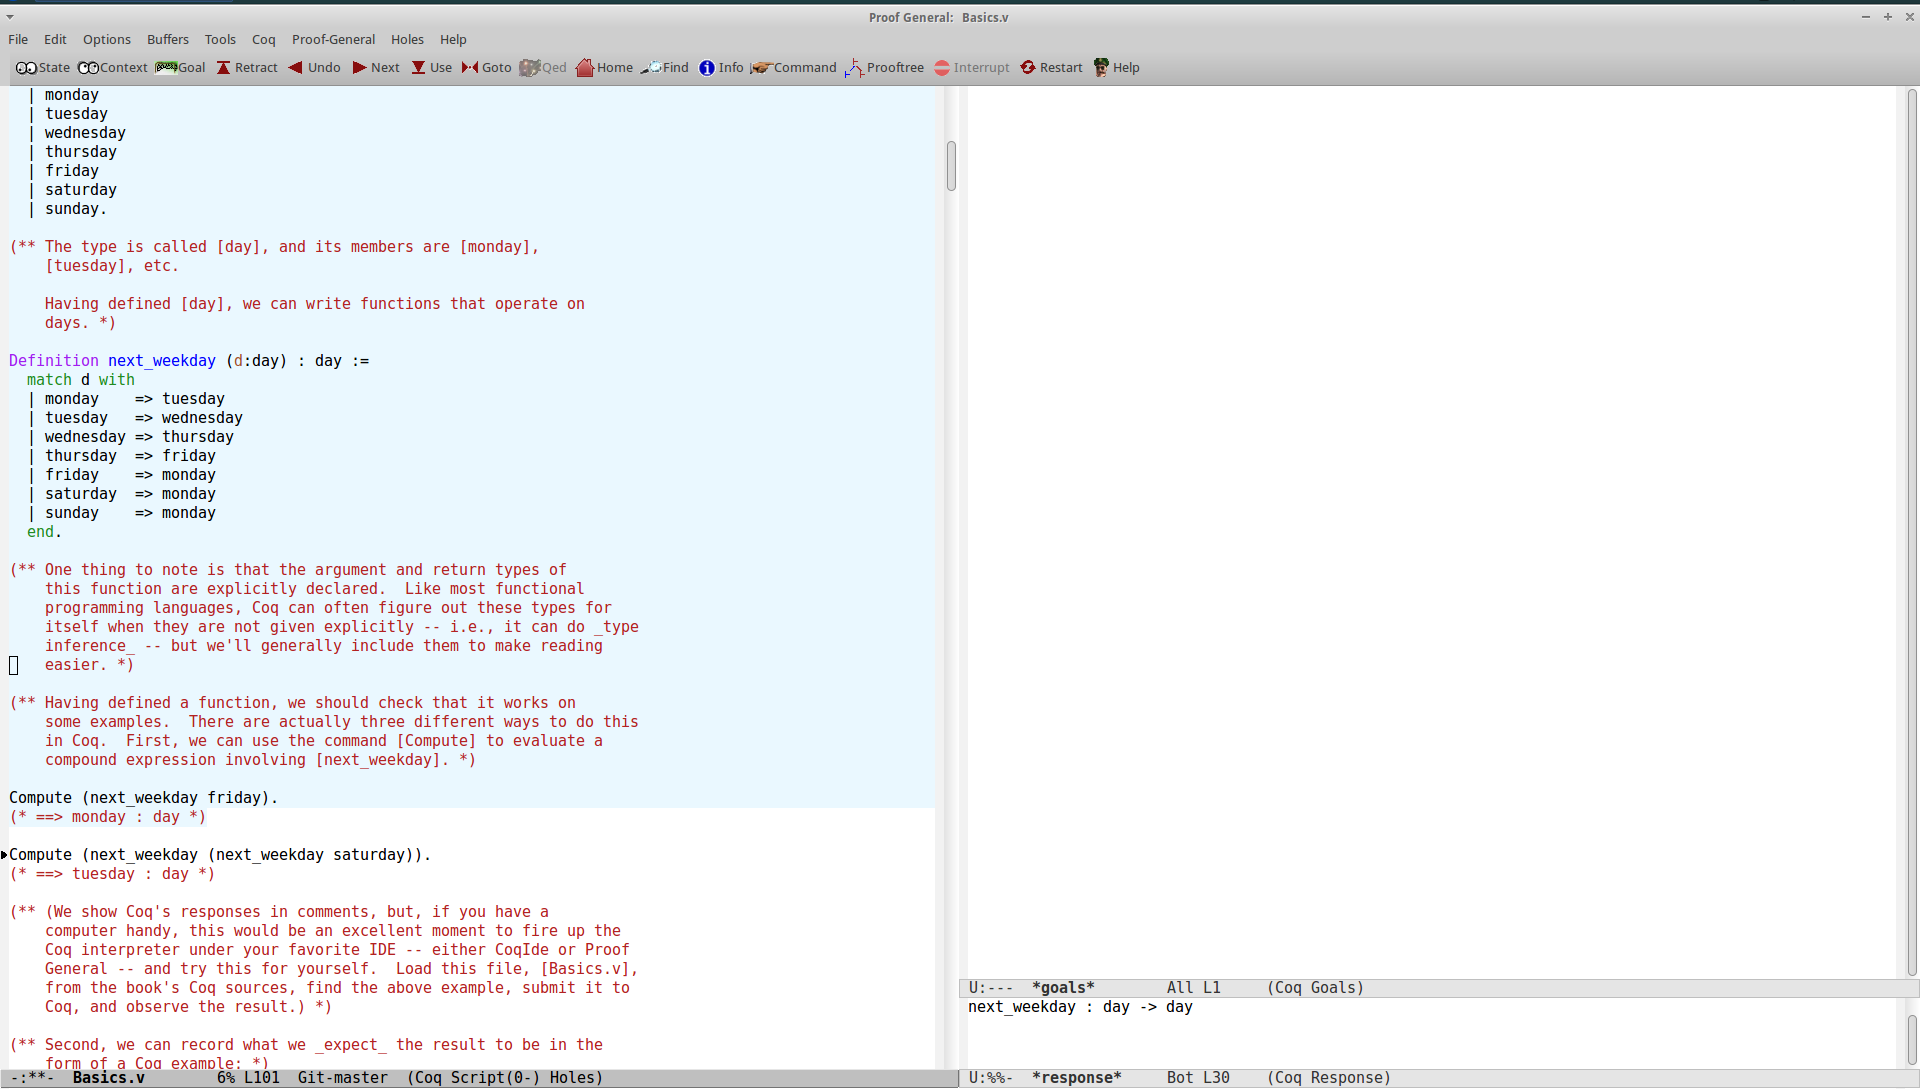
\includegraphics[width=.9\textwidth]{proofgeneral.png}
	%		\label{fig:screenshot-proof-general}
	%		\caption{Coq interface in proof general.}
	%	\end{figure}    
    	
	\end{frame}

	
	
	% Let's talk about verifiying an OS
	% Maroon
	% was kann das
	% wie groß ist das
	% ihr baut andauernd daran rum?
	% das Betreibssystem aus dem Airbus?
	
   % Linux Realtime Patch?   MPI-SWS hat einen.	
	
	
	% let's talk about Ada- and Maroon
	% LOC Ada code
	% LOC Marron Scheduler
	
	% Kaiser's Scheduler? 
	% I don't know
	% Wurde der nicht verkauf?
	% Können wir den noch benutzen?
	
	
	
	
%%%%%%%%%%%%%%%%%%%%%%%%%%%%%%%%%%%%%%%%%%%%%%%%%%%%%%%%%%%%%%%%%%%%%%%%%%%%%%%%%%%%%% 
% Books 
%%%%%%%%%%%%%%%%%%%%%%%%%%%%%%%%%%%%%%%%%%%%%%%%%%%%%%%%%%%%%%%%%%%%%%%%%%%%%%%%%%%%%%%	
	
	\begin{frame}{Bibliography}
		\begin{thebibliography}{10}
		\beamertemplatebookbibitems
		
		
		\bibitem{PACGGHSY2019}
		B. C.~ Pierce and A. A.~de Amorim and C.~Casinghino and M.~Gaboardi and M.~Greenberg and C.~Hriţcu and V.~Sjöberg and B.~Yorgey
		\newblock \doublequoted{Software Foundations, Logical foundations, Volume 1}
		\newblock \url{https://softwarefoundations.cis.upenn.edu/current/lf-current/index.html}, 2019
			
		\bibitem{COQ}
		Coq- Project Website	
		\newblock \doublequoted{The Coq Proof Assistant}
		\newblock \url{https://coq.inria.fr} , 2019-01-09
		
		
		\bibitem{RTproofs}
		RT-Proofs Website
		\newblock \doublequoted{Formal Proofs for Real-Time Systems}	
		\newblock \url{https://rt-proofs.inria.fr}, 2020-14-02		
		\end{thebibliography}	
	\end{frame}	
	
%%%%%%%%%%%%%%%%%%%%%
% IDES bibliography
%%%%%%%%%%%%%%%%%%%%%	

	\begin{frame}{Bibliography}{Coq}
		\begin{thebibliography}{10}
		\beamertemplatebookbibitems
		
		\bibitem{coqide}
		Coq Integrated Development Environment - Offical Documentation
		\newblock \doublequoted{Coq Integrated Development Environment}
		\newblock \url{https://coq.inria.fr/refman/practical-tools/coqide.html}		
				
		\bibitem{PG}
		Proof General - Project Website
		\newblock \doublequoted{Proof General, a generic interface for proof assitants.}
		\newblock \url{https://proofgeneral.github.io/}, 2020-14-02
		
		\bibitem{coquille}
		Coquille - Andreas Werner's Fork
		\newblock \doublequoted{Coquille, a vim plugin.}
		\newblock \url{https://github.com/Werner2005/coquille}, 2020-14-02		
		\end{thebibliography}
	\end{frame}
	
	
%%%%%%%%%%%%%%%%%%%%%%
% Coq online  	
%%%%%%%%%%%%%%%%%%%%%%

\begin{frame}{Bibliography: Online}
	\begin{thebibliography}{10}
		\beamertemplatebookbibitems
		
		\bibitem{syntaxhighliting}		
		N. Giannarakis
		\newblock Coq - Syntax Highlithing
		\newblock \doublequoted{Personal GitHub Profile}
		\newblock \url{https://github.com/nickgian/thesis/lstcoq.sty}, 2019-19-09		

	
		
		\end{thebibliography}
	
\end{frame}		
	
%%%%%%%%%%%%%%%%%%%%%%%%%%%%%%%%%
% Real-Time Systems
%%%%%%%%%%%%%%%%%%%%%%%%%%%%%%%%%%


	\begin{frame}{Bibliography: Real-Time Systems}
		\begin{thebibliography}{10}
			\beamertemplatebookbibitems
			
		
			\bibitem{KBK}		
			R. Kaiser and K. Beckmann and R. Kröger
			\newblock \doublequoted{Echtzeitplanung}
			\newblock Handouts \url{https://www.cs.hs-rm.de/~kaiser/1919_ezv/6_Scheduling-handout.pdf} 2020-07-01
			
			\bibitem{L}
			J. W.S. Liu
			\newblock \doublequoted{Real-time Systems}
			\newblock Prentice-Hall, Inc., ISBN: 0-13-099651-3, 2000
			
			\bibitem{K}
			R. Kasier 
			\newblock \doublequoted{Virtualisierung von Mehrprozessorsystemen mit Echtzeitanwendungen}
			\newblock PHD Thesis, Universität Koblenz-Landau, 11-02-2009
		\end{thebibliography}
	
	\end{frame}		
	

\begin{frame}{Bibliography: Real-Time Systems}
	\begin{thebibliography}{10}
		\beamertemplatebookbibitems		
		
		\bibitem{B}
		G. Bollella 
		\newblock \doublequoted{Slotted Priorities: Supporting Real-Time Computing Within General-Purpose Operating Systems}
		\newblock PHD Thesis, Chapel Hill, 1997	
	
	    
	   	\beamertemplatearticlebibitems
	    
	    \bibitem{C}
	    M. Bertogna and M. Cirinei
	    \newblock \doublequoted{Response-Time Analysis for Globally Scheduled Symmetric Multiprocessor Platforms}
	    \newblock Proceedings of the 28th IEEE International Real-Time Systems Symposium (RTSS 07)
	    
			\end{thebibliography}
	    
  


\end{frame}		



%%%%%%
% Conference Papers
%%%%%%
		
	
%@InProceedings{10.1007/978-3-030-25543-5_28,
%	author="Guo, Xiaojie and Lesourd, Maxime and Liu, Mengqi and Rieg, Lionel and Shao, Zhong",
%	editor="Dillig, Isil
	%and Tasiran, Serdar",
	%title="Integrating Formal Schedulability Analysis into a Verified OS Kernel",
	%booktitle="Computer Aided Verification",
	%year="2019",
	%publisher="Springer International Publishing",
	%address="Cham",
	%pages="496--514",
	%abstract="Formal verification of real-time systems is attractive because these systems often perform critical operations. Unlike non real-time systems, latency and response time guarantees are of critical importance in this setting, as much as functional correctness. Nevertheless, formal verification of real-time OSes usually stops the scheduling analysis at the policy level: they only prove that the scheduler (or its abstract model) satisfies some scheduling policy. In this paper, we go further and connect together Prosa, a verified schedulability analyzer, and RT-CertiKOS, a verified single-core sequential real-time OS kernel. Thus, we get a more general and extensible schedulability analysis proof for RT-CertiKOS, as well a concrete implementation validating Prosa models. It also showcases that it is realistic to connect two completely independent formal developments in a proof assistant.",
	%isbn="978-3-030-25543-5"
	%}		
	%
	%
	%
	%
	%
	%
	%

%%%%%%%%%%%%%%%%%%%%%%%%%%%%%%%%%%%%%%%%%%%%%%%%%%%%%%%%
% Operating Systems Literature
%%%%%%%%%%%%%%%%%%%%%%%%%%%%%%%%%%%%%%%%%%%%%%%%%%%%%%%%
		
	\begin{frame}{Bibliography: Real-Time Systems}
		\begin{thebibliography}{10}
		\beamertemplatebookbibitems
		
		\bibitem{PROSA_ECRTS16ArtifcatEvaluation}
		F.~ Cerqueira and  F. ~ Stutz, and B.~ Brandenburg
		\newblock \doublequoted{Prosa - ECRTS’16 Artifact Evaluation}
		\newblock \url{https://prosa.mpi-sws.org/releases/v0.1/artifact/},  2020-01-09
		
		\beamertemplatearticlebibitems
		
		\bibitem{PROSA_schedubility_analysis }		
		F.~ Cerqueira and  F. ~ Stutz, and B.~ Brandenburg		
		\newblock \doublequoted{PROSA: A Case for Readable Mechanized Schedulability Analysis}	
		\newblock \url{https://www.mpi-sws.org/~bbb/papers/pdf/ecrts16f.pdf}
		\newblock Proceedings of the 28th Euromicro Conference on Real-Time Systems (ECRTS), 2016	
		\end{thebibliography}	
	\end{frame}		
	
%%%%%%%%%%%%%%%%%%%%%%%%%%%%%%%%%%%%%%%%%%%%%%%%%%%%%%%
% Compiler Stuff
%%%%%%%%%%%%%%%%%%%%%%%%%%%%%%%%%%%%%%%%%%%%%%%%%%%%%%%%
	
	\begin{frame}{Bibliography: Computer and Communication Security}
		\begin{thebibliography}{10}
			\beamertemplatearticlebibitems
		
			\bibitem{JASMIN}
		Almeida, Jos\'{e} Bacelar and Barbosa, Manuel and Barthe, Gilles and Blot, Arthur and Gr\'{e}goire, Benjamin and Laporte, Vincent and Oliveira, Tiago and Pacheco, Hugo and Schmidt, Benedikt and Strub, Pierre-Yves
			\newblock \doublequoted{Jasmin: High-Assurance and High-Speed Cryptography}
			\newblock Proceedings of the 2017 ACM SIGSAC Conference on Computer and Communications Security (CCS), 2017
		\end{thebibliography}
	 \end{frame}
	 
	
	 
	% Examples from latex Template	
	%	\beamertemplatearticlebibitems
		
		
	%	\beamertemplatebookbibitems
	%	\bibitem{Oppenheim2009}
	%	Alan~V.~Oppenheim
	%	\newblock \doublequoted{Discrete-Time Signal Processing}
	%	\newblock Prentice Hall Press, 2009
	%
	%	\beamertemplatearticlebibitems
	%	\bibitem{EBU2011}
	%	European~Broadcasting~Union
	%	\newblock \doublequoted{Specification of the Broadcast Wave Format (BWF)}
	%	\newblock 2011
	


\end{document}






